%https://medemanabu.net/latex/documentclass/
\documentclass[12pt,oneside]{jbook}
%\documentclass[a4j,12pt,oneside]{jbook}
\usepackage{master_thesis2020}
\usepackage{comment}
\usepackage{amssymb}

%https://www.overleaf.com/learn/latex/Nomenclatures
\usepackage{nomencl}
\makenomenclature
\usepackage{etoolbox}
\renewcommand\nomgroup[1]{%
  \item[\bfseries
  \ifstrequal{#1}{A}{Physics Constants}{%
  \ifstrequal{#1}{B}{Material Properties}{%
  \ifstrequal{#1}{C}{Other Symbols}{}}}%
]}
\newcommand{\nomunit}[1]{%
\renewcommand{\nomentryend}{\hspace*{\fill}#1}}


\begin{document}
\thesistitle
	{Forced convective heat transfer in cylindrical pipe flows} % 論文題目
	{MD18060} % 学籍番号
	{Yoshinori}{Hattori} % 氏名
    {}{}
\tableofcontents

\mbox{}
\nomenclature[A, 02]{$c$}{Speed of light in a vacuum inertial system\nomunit{$299,792,458\, m/s$}}
\nomenclature[A, 03]{$h$}{Plank Constant\nomunit{$6.62607 \times 10^{-34}\, Js$}}
\nomenclature[B, 01]{$T$}{Temperature\nomunit{$K$}}
\nomenclature[B, 02]{$C_{p}$}{Specific heat capasity\nomunit{$J \cdot kg^{-1} K^{-1}$}}
\nomenclature[B, 03]{$\lambda$}{Thermal conductivity\nomunit{$W m^{-1} K^{-1}$}}
\nomenclature[B, 04]{$\mu$}{Dynamic viscosity\nomunit{$Pa \cdot s$}}
\nomenclature[B, 05]{$\rho$}{Density\nomunit{$kg/m^{3}$}}
\nomenclature[B, 06]{$Pr$}{Prandtl number\nomunit{-}}

\nomenclature[C]{$V$}{Constant Volume}
\nomenclature[C]{$\rho$}{Friction Index}
\printnomenclature

\chapter{Introduction}
\section{Study background}
Forced convective heat transfer lies at the heart of many aspect of cooling technology and it is therefore desirable to understand its properties as well as possible.
Effective cooling technology is constantly being required to wide variety of industrial engineering aplication.
To achieve effective coolant system requires comprefensive research of heat transfer coefficient with a wide variety of flow condition.
Although many reserchers have been focusing on experimental and computational research, heat transfer coefficient vary with Reynolds number is still unclear.
To this end, many reserchers have been focusing on heat transfer from experimental and computational research aspect.
However, heat transfer in transitional and turbulent flow is still very challenging task for both experimental and computational research.
\begin{enumerate}
	\item Experimental research\\

	\item Computational research\\
	Direct numerical simuration
	In technology, flows regime and heat transfer plays an important role in considerting engineering issues.
	Navie-Stokes equations describe the relation of variable flows.
	\begin{equation}
		\
	\end{equation}
	However, deterministic solution of the equations are only valid for small disturbances in the initial and boundary condition.
	In physically, it is hard to get initial and boundary conditions in infinite accurate.
	Turbulent has a large amount of fluctuations, i.e. turbulent is completely different kind of laminar flows.
	Direct Numerical Simuration (DNS) is one of the simulation way to predict flow forms.
	The object of the simuration is to solve the compelete set of equation of motion without using any model.
	From Kolmogorov lenght scale, total number of cumputations is derivered following equation (\ref{DNS_total_number_of_computation}).
	The DNS require large amount of total number of computations.
	\begin{equation}
	    \mathcal N \times \mathcal M= \mathcal O (Re^{11/4})
	    \label{DNS_total_number_of_computation}
	\end{equation}
	The equauation implies the limitation of the DNS and that is directly connected to computer technology.
	Normally, engineeres is interested in high Reynolds number such as aircraft or atmospheric boundary layer.
	However, such high Reynolds number requires huge amount of total number of computations and it's far from reality.
	Large eddy simulation
\end{enumerate}

One attempt to improve our understanding of entanglement is the study of our ability to perform experimental investigation


These coolant technology is used wide varaety of coolant applications such as electric devices, automotive, and plant factory.
Considering heat transfer issues, heat transfer coefficients are one of the most important numbers.
The Nusselt number (Nu) is a dimensionless number which represents the ratio of convective (h) and conductive heat transfer (k), as expressed in Equation.
\section{Previous research}

The equauation implies the limitation of the DNS and that is directly connected to computer technology.
Normally, engineeres is interested in high Reynolds number such as aircraft or atmospheric boundary layer.
However, such high Reynolds number requires huge amount of total number of computations and it's far from reality.

Therefore, it is nessesary to get experimental data for correlations of heat transfer and flow condition and the Reynolds number.

%attention!!!!!!!!!!!
Many studies have pointed out that a heat transfer coefficient varies depending on the type of flow: laminar, transition and turbulent.
Gnienlinski\cite{Gnielinski1975} showed a calculation method about heat transfer coefficients for the laminar, transitional and turbulent flows.
Bertsche et al.\cite{Bertsche2016} focused on reliable prediction of the heat transfer coefficient for transitional flows.
In their study, they showed experimental the heat transfer coefficients for the Reynolds number, $500 < Re < 23000$, and the Prandtl number, $7 < Pr < 41$.\\
However, not so many data is available for experimental data of laminar-to-turbulent transitional region.
More studies should be conducted to obtain experimental data for high the Prandtl number and transitional flows.
In this study, the author focused on forced convective heat transfer in flow of water and glycole in a cylindrical pipe.
A 50/50vol\% mixture of water and glycole, which is a typical liquid coolant in automotive applications, was used as an operating fluid.
The experiment was carried out by considering a board range of Reynolds numbers, spanning from a laminar to fully turbulent flow.
Moreover, the measurements of the wall friction coefficients was also performed in this study.

\subsection{Skin friction coefficients}
The skin friction coefficients for laminar flow is descrived following equation.
\begin{equation}
    C_{f,lam}=\frac{16}{Re_{b}}
    \label{cf_laminar}
\end{equation}

Konakov\cite{Petukhov1970} showed the skin friction coefficients for turbulent flow.
\begin{equation}
	C_{f,turb}=0.25(1.8log(Re_{b})-1.64)^{-2}
	\label{cf_turbulent}
\end{equation}

\subsection{The heat transfer coefficients}
Gunienski \cite{Gnielinski2013} showed correlations for each flow conditions: laminar, transitional and turbulent, respectively.
Gunienski \cite{Gnielinski2013} showed calculation method for laminar flow.
\begin{equation}
    Nu_{lam}=(3.66^{3}+0.7^{3}+(1.615(Re_{b}Pr_{b}\frac{d_{i}}{L})^{1/3})^{3})^{1/3}
    \label{Nu_laminar}
\end{equation}
%The range 0.1<<Pr_{b}<<1000, 10^{4}<<Re_{b}<<10^{6}.
He showed calculation method for turbulent flow.
\begin{equation}
    Nu_{turb}=\frac{\frac{C_{f,turb}}{2Re\cdot Pr_{b}}}{1+12.7 \sqrt{\frac{C_{f,turb}}{2}}(Pr_{b}^{2/3}-1)}\cdot (\frac{Pr_{b}}{Pr_{w}})^{0.11}
    \label{Nu_turbulent}
%Nu_{turb}=\frac{\frac{C_{f}}{2\cdot Re\cdot Pr_{b}}{(1+12.7\frac{C_{f}}{2}}\cdot (Pr^{\frac{2}{3}}-1)}\cdot(1+(\frac{d_{h}}{l})^{\frac{2}{3}})\label{Nu_turblent}
\end{equation}
The range is
\begin{equation}
    0.1<<Pr_{b}<<1000, 10^{4}<<Re_{b}<<10^{6}
\end{equation}
He presented transitional flow as a liner interpolation between turbulent and laminar flow.
\begin{equation}
    Nu_{m}=(1-r)Nu_{m,lam}+rNu_{m,turb}
    \label{Nu_transitional}
\end{equation}
\begin{equation}
    r=\frac{Re_{b}-2300}{10^{4}-2300}
	\label{Nu_transitional2}
\end{equation}

\chapter{Methodology}
\section{Material properties}
A 50/50vol\% mixture of water and glycole which is a typical liquid coolant in automotive applications were used as a operating fluid.

specific heat capacity
\begin{equation}
	c_{p} = A_{c_{p}}+B_{c_{p}} T = 2.0148 + 4.50E-3T
	\label{Cp}
\end{equation}
\begin{figure}[ht]
	\vspace{0zh}
	\begin{center}
		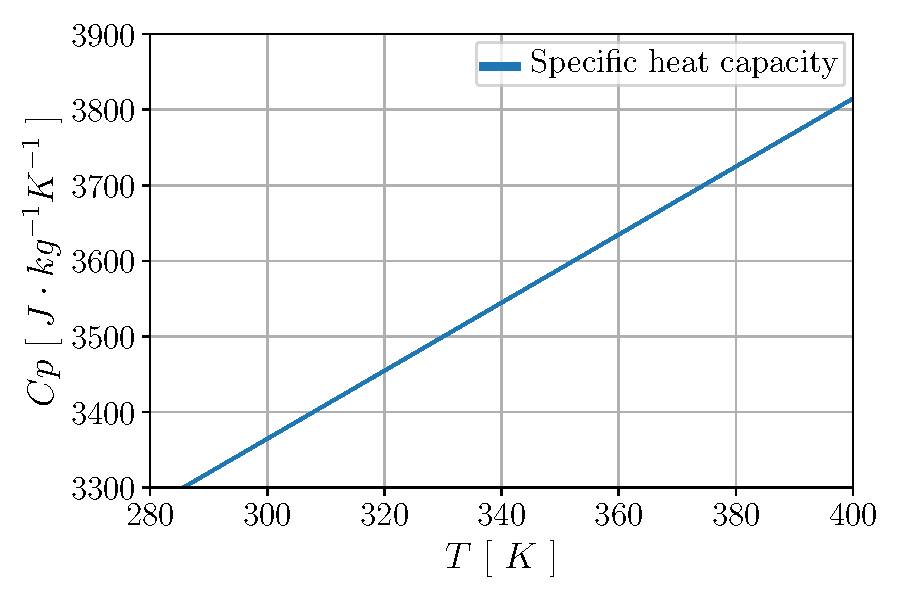
\includegraphics[width=0.65\linewidth]{fig/cp.pdf}
		\vspace{-1zh}
		\caption{Specific heat capacisty vary with temperature}
		\label{cp}
	\end{center}
	\vspace{0zh}
\end{figure}


thermal condictivity
\begin{equation}
	\lambda = A_{\lambda}+B_{\lambda} T = 0.2134 + 6.071E-4T
	\label{lambda}
\end{equation}
\begin{figure}[ht]
	\vspace{0zh}
	\begin{center}
		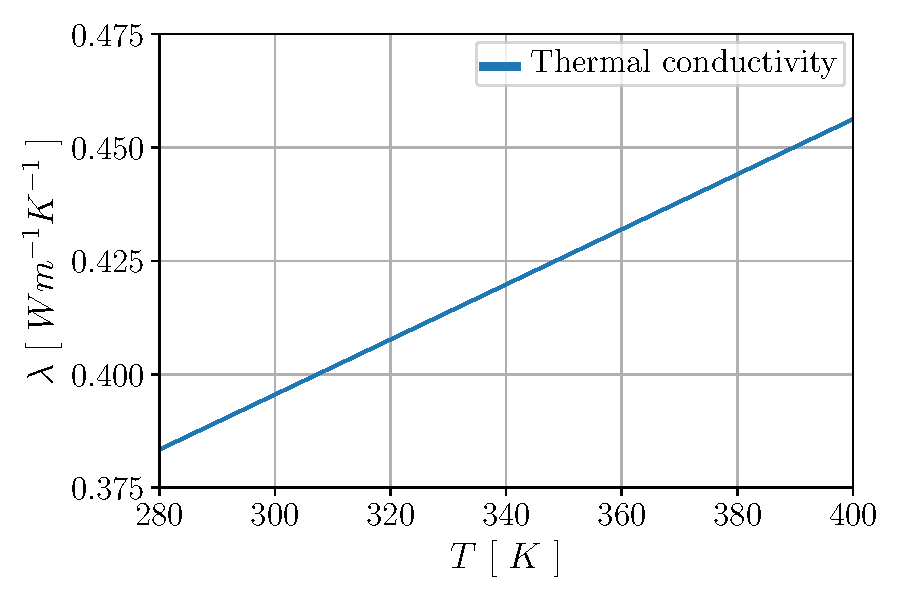
\includegraphics[width=0.65\linewidth]{fig/lambda.pdf}
		\vspace{-1zh}
		\caption{Thermal conductivity vary with temperature}
		\label{lambda}
	\end{center}
	\vspace{0zh}
\end{figure}


dynamic viscosity
\begin{equation}
	\mu = A_{\mu}\cdot \exp \left( \frac{B_{\mu}}{T+C_{\mu}} \right) = 1.1001E-4\exp \left( \frac{325.85}{T-207.30} \right)
	\label{mu}
\end{equation}
\begin{figure}[ht]
	\vspace{0zh}
	\begin{center}
		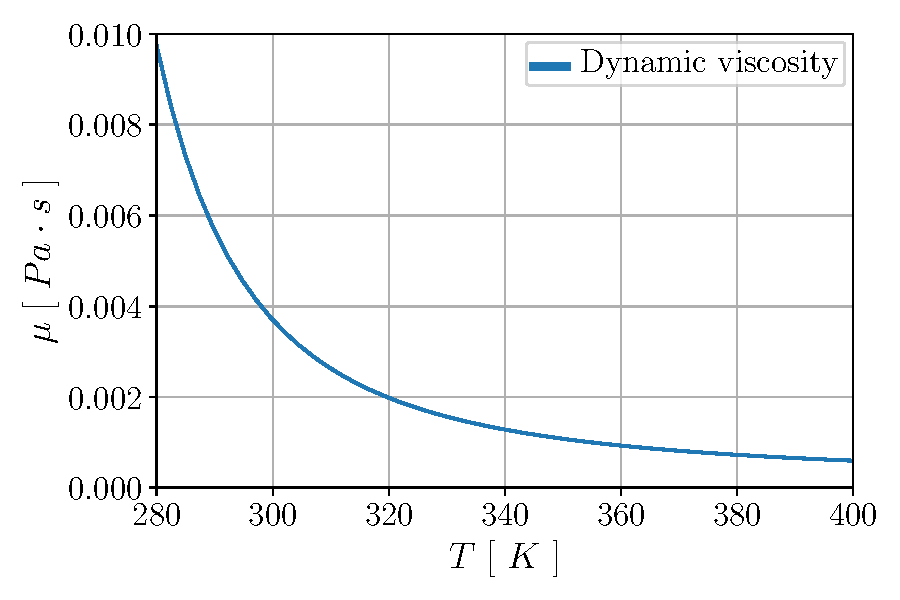
\includegraphics[width=0.65\linewidth]{fig/mu.pdf}
		\vspace{-1zh}
		\caption{Dynamic viscosity vary with temperature}
		\label{mu}
	\end{center}
	\vspace{0zh}
\end{figure}


density
\begin{equation}
	\rho = A_{\rho}+B_{\rho} T = 1268.28 -0.66T
	\label{rho}
\end{equation}
\begin{figure}[ht]
	\vspace{0zh}
	\begin{center}
		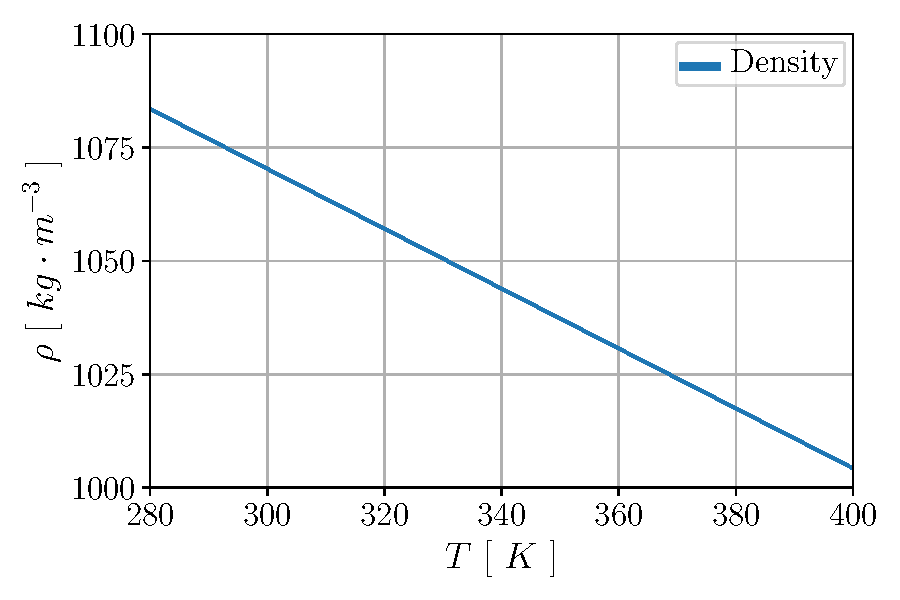
\includegraphics[width=0.65\linewidth]{fig/rho.pdf}
		\vspace{-1zh}
		\caption{Density vary with temperature}
		\label{rho}
	\end{center}
	\vspace{0zh}
\end{figure}


prandtl number
\begin{equation}
	Pr = \frac{\nu}{\alpha}= \frac{\mu \cdot c_{p}}{\lambda}
	\label{pr}
\end{equation}
\begin{figure}[ht]
	\vspace{0zh}
	\begin{center}
		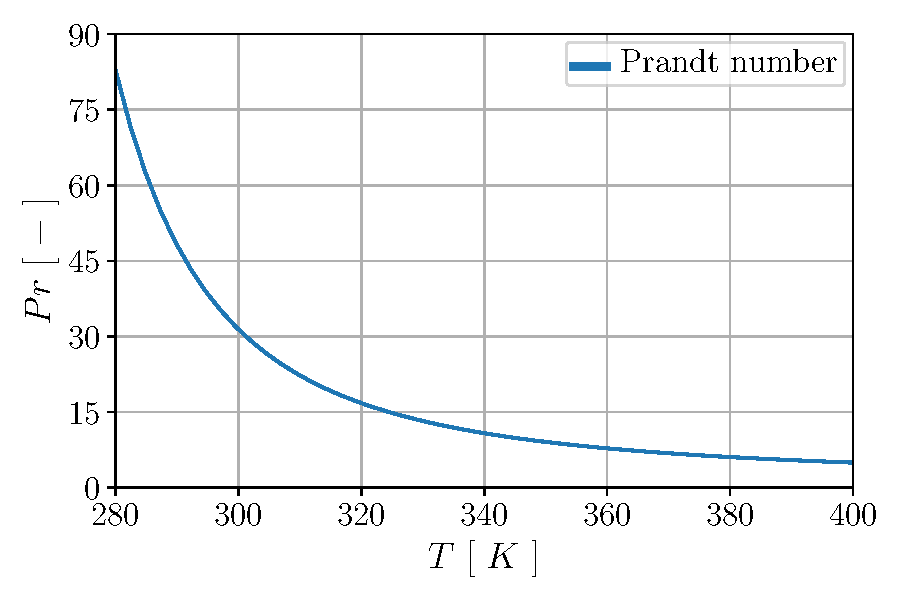
\includegraphics[width=0.65\linewidth]{fig/pr.pdf}
		\vspace{-1zh}
		\caption{Prandtl number vary with temperature}
		\label{pr}
	\end{center}
	\vspace{0zh}
\end{figure}

\clearpage
\section{Hydro and thermal boundary layer}

\chapter{Experimental facilities}
\section{Experimental loop}
\section{Test section}
\section{Wall temperature distribution}
\section{Evaluation procedure}
\section{Measurement Uncertainty}

\chapter{Experiments}
\section{Validity of Experimental and evaluation procedure}
\section{Experimental result and variation}
\subsection{Validation of experimental result for $Pr_{w}=7$}
\subsection{Validation of experimental result for $Pr_{w}=10$}
\subsection{Validation of experimental result for $Pr_{w}=13$}

\section{Discussion}
\subsection{Reproducibility}
\subsection{Influence of heat flux}
\subsection{Scattering and proberbility density function}
\subsection{Comparison with DNS and LES}
\chapter{Conclusion}


\appendix
% !TEX root = ../thesis-sample.tex
\appendix
\doublespacing
\chapter{Material properties}
A 50/50vol\% mixture of water and glycole which is a typical liquid coolant in automotive applications were used as a operating fluid.

\chapter{Post processing}
\lipsum[24]


%http://lightology.hatenablog.com/entry/2018/02/12/221721
\bibliographystyle{amsplain}
\bibliography{/Users/Shared/TeXLive/texmf/bibtex/bib/local/graz.bib}
%\bibitem{Frank}Frank P.Incropera et al., ``Fundamentals of Heat and Mass Transfer'', (Wiley, 2006)

\end{document}
